\documentclass{jlreq}
\usepackage{graphicx}
\usepackage{amsmath,amssymb,mathtools,bm}
\usepackage{siunitx}
\sisetup{per-mode=symbol}
\usepackage{physics}
\usepackage{mhchem}
\usepackage{booktabs}
\usepackage{ascmac}
\usepackage{hyperref}
\hypersetup{colorlinks=true,linkcolor=black,urlcolor=blue,citecolor=black}
\usepackage{enumitem}
\usepackage{geometry}
\usepackage{caption}
\usepackage{makecell} % ← セル内改行・回転文字用


% ===== Title =====
\title{角運動量保存則}
\author{学籍番号：2225091~~~~~~氏名 : 西亦 岳雄}

\begin{document}

\maketitle

% ===== 目的 =====

\begin{itembox}[l]{\large 実験の目的}

　今回の実験では, 錘を取り付けた地球ゴマに
外力のモーメント$\bm{N} = \bm{r} \times \bm{F}$を与えたときの歳差運動から,
その外力のモーメントと角速度$\bm{\Omega}$を調べることで角運動量が
どのように変化するかを理解する.

\end{itembox}



% ===== 原理 =====
\section*{1.原理}

\subsubsection*{1.1.回転と並進}
力のモーメントと角運動量を導入する前に, 回転について考える. 
図1のように, 点Pにある物体に力$\bm{F}$が働いている状況を考える. 
すると, 力$\bm{F}$はOPに平行な成分と垂直な成分に分けられ, 
これがそれぞれ並進と回転という作用である. 垂直な成分, つまり回転は
OPに対して角度を与える方向の作用であることがわかる. 


\begin{figure}[hbtp]
  \centering
  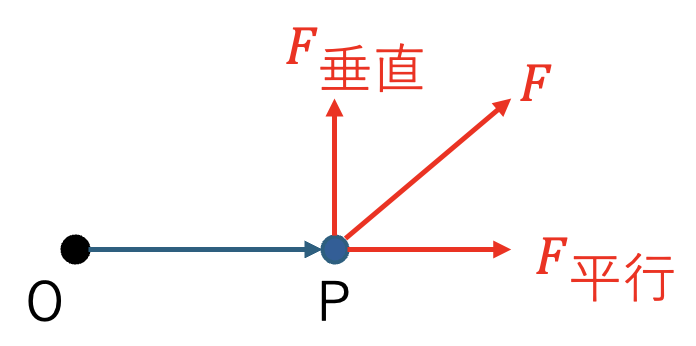
\includegraphics[width=0.5\linewidth]{images/number1.png} % ← 拡張子・大文字小文字に注意！
  \caption{並進と回転}
\end{figure}

\subsubsection*{1.2.力のモーメント}
回転の運動に関して, 回転軸に注目して, 回転の作用方向を回転に沿って
右ねじを回したときに進む方向で定義する. このときに, 回転作用の大きさと
方向を表すベクトル量として力のモーメント(トルク)を導入する. \par

図2のように原点Oを基準点とする場合, 力のモーメント(トルク)は
\begin{align}
    \bm{N} = \bm{r} \times \bm{F}
\end{align}
と定義される. トルクの大きさは
\begin{align}
    N = |\bm{r} \times \bm{F}| = rF\sin \theta
\end{align}
で, トルクの方向は図2のように$z$軸方向である. 


\begin{figure}[hbtp]
  \centering
  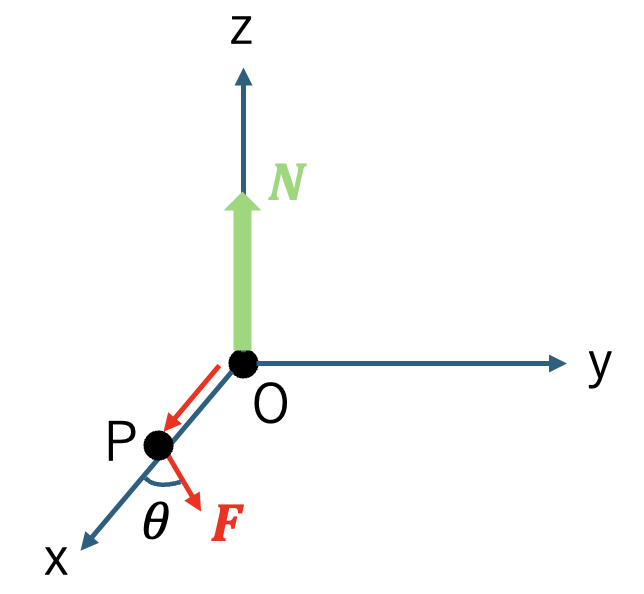
\includegraphics[width=0.5\linewidth]{images/number2.png} % ← 拡張子・大文字小文字に注意！
  \caption{力のモーメント}
\end{figure}



\subsubsection*{1.3.角運動量}

角運動量は, 回転運動の大きさとその方向を表すベクトル量であり, 
図3のように原点Oのまわりの角運動量$\bm{L}$は
\begin{align}
    \bm{L} = \bm{r} \times \bm{p}
\end{align}
と書ける.

\begin{figure}[hbtp]
  \centering
  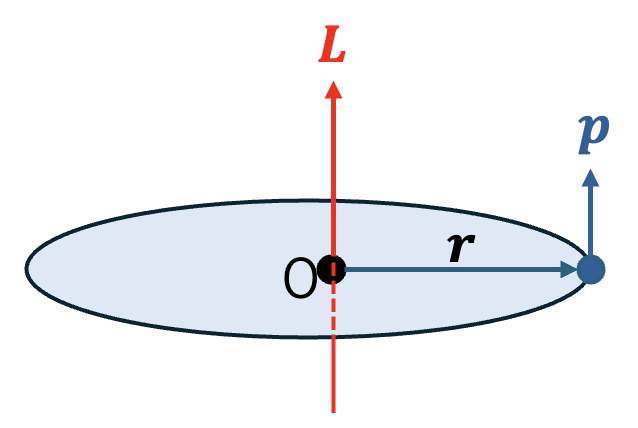
\includegraphics[width=0.5\linewidth]{images/number3.png} % ← 拡張子・大文字小文字に注意！
  \caption{角運動量}
\end{figure}


\subsubsection*{1.3.角運動量とトルクの関係}

角運動量の時間微分を考えて
\begin{align}
    \dot{\bm{L}} &= \left[\frac{d}{dt} (\bm{r} - \bm{r_0})\right] \times \bm{p} + (\bm{r} - \bm{r_0}) \times \frac{d\bm{p}}{dt}\\
                 &= \bm{v} \times \bm{p} + (\bm{r} - \bm{r_0}) \times \bm{F}\\
                 &= \bm{v} \times (m\bm{v}) + (\bm{r} - \bm{r_0}) \times \bm{F}\\
                 &= (\bm{r} - \bm{r_0}) \times \bm{F}\\
                 &= \bm{N}
\end{align}
が成り立ち, 質点に働く力$\bm{F}$が$\bm{r}$と平行または0のとき
\begin{align}
    \dot{\bm{L}} = 0
\end{align}
で角運動量保存則が導かれる.


\subsubsection*{1.3.慣性モーメント}
剛体とは, 外力がかかっても変形しない理想的な物体のことである. その剛体の運動を記述するため, 剛体の運動方程式を立てる. まず, ある剛体に軸を指し, その軸を指定するためにある2点を決める必要がある(この状態だと軸の周りに剛体が回転できてしまう). ここで, 剛体中のもう一点を指定し固定すれば剛体の刻々の動きを決めることができる. この一点は, $x,y,z$座標の三つのパラメータで決まるので, ここまでで9つのパラメータを指定する必要がある. さらに, 剛体を貫く2点と剛体の回転を止めるための残りの1点の互いの距離を一定とすれば, 自由度は6となり以下の6つの方程式を決めることができる.
\begin{align}
    M \ddot{\bm{r}}_G = \sum_{i=1}^{n} \bm{F}_i
\end{align}

\begin{align}
\bm{N} = \sum_{i=1}^{n} \bm{r}_i \times \bm{F}_i
\end{align}
ただし, $M$:剛体の質量, $\bm{r}_G$:剛体の重心の位置, $\bm{N}$:原点周りのトルク, $\bm{F}_i$:剛体中の$i$番目の質点が受ける外力である.
　剛体が固定された軸に貫かれている場合を考える. このときの剛体の自由度は1となるから, 必要な方程式は1つとなる. また, 剛体の運動は固定軸($z$軸)回りのトルクを用いて
\begin{align}
    N_z = \dot{L}_z
\end{align}
の式に従う. 剛体を微小な立方体に分割し$L_z$に関して足し上げると
\begin{align}
    L_z &= \sum_{i=1}^{n} (\bm{r}_i \times \bm{p}_i)\\
        &= \sum_{i=1}^{n} (\bm{r}_i \times m_i \dot{\bm{r}}_i)_z\\
        &\xrightarrow[\Delta V \to 0]{} \int_{}^{} dV[\bm{r} \times \rho(\bm{r})\dot{\bm{r}}]_z
\end{align}
ただし, $dV$:微小体積, $\rho(\bm{r})$:位置$\bm{r}$での密度である. ここからは, 円筒座標系を用いて(3)における角運動量を求める. 底面が$x,y$平面にあり, 中心軸を$z$軸とする円筒を考える. 底面の半径を$\xi$, $x$軸から$\xi$までの角度を$\theta$, $\xi, \theta, z$で指定される位置ベクトルを$\bm{r}$とする. すると,
\begin{align}
    \bm{r} \times \dot{\bm{r}} &= (\xi \bm{e}_{\xi} + z \bm{e}_z) \times \frac{d}{dt}(\xi \bm{e}_{\xi} + z \bm{e}_z)\\
                               &= (\xi \bm{e}_{\xi} + z \bm{e}_z) \times (\xi \dot{\bm{e}}_{\xi} + \xi \dot{\bm{e}}_{\xi} + \dot{z} \bm{e}_z)\\
                               &= (\xi \bm{e}_{\xi} + z \bm{e}_z) \times (\xi \dot{\bm{e}}_{\xi} + \xi \dot{\theta} \bm{e}_{} + \dot{z} \bm{e}_z)\\
                               &= (-z \xi \dot{\theta}) \bm{e}_{\xi} + (z \dot{\xi} - \xi \dot{z}) \bm{e}_{\theta} + ({\xi}^2 \dot{\theta}) \bm{e}_z
\end{align}
から, 角運動量の$z$成分は
\begin{align}
    L_z &= \int_{}^{} dV [\bm{r} \times \rho(\bm{r}) \dot{\bm{r}}]_z\\
        &= \int dV [\rho(\bm{r}) {\xi}^2 \dot{\theta}]\\
        &= \dot{\theta} \int_{}^{} dV [\rho(\bm{r}) {\xi}^2]
\end{align}
となり, $\int_{}^{} dV [\rho(\bm{r}) {\xi}^2]$の部分を$I_z$として慣性モーメントとする. (13)式について両辺を時間微分すると
\begin{align}
    \dot{L_z} = N_z = I_z \ddot{\theta}
\end{align}
が成り立つ.
　また, 運動エネルギー$K$に関して,
\begin{align}
    K &= \sum_{i=1}^{n} \frac{1}{2} m_i {\dot{\bm{r}}_i}^2\\
      &= \sum_{i=1}^{n} \frac{1}{2} m_i (\dot{\xi}_i \bm{e}_{\xi} + \xi_i \dot{\theta}_i \bm{e}_{\theta} + \dot{z_i} \bm{e}_z)^2\\
      &= \sum_{i=1}^{n} \frac{1}{2} m_i (\xi_i \dot{\theta}_i)^2\\
      & \xrightarrow[\Delta V \to 0]{} \int dV \frac{1}{2} \rho(\bm{r}) (\xi \dot{\theta})^2\\
      &= \frac{1}{2} I_z \dot{\theta}^2
\end{align}
が成り立つ.


% ===== 実験装置構成・実験手順 =====
\section*{2.実験装置構成・実験手順}


% ===== 結果と解析 =====
\section*{3.結果と解析}


% ===== 考察 =====
\section*{4.考察}


% ===== 概括 =====
\section*{5.概括}





\end{document}